\documentclass[conference]{IEEEtran}
\pdfoutput=1    % For arXiv issues


% -------------------------- COLORBLIND COLORS -------------------------------
% Use color palettes for colorblind people from
% https://davidmathlogic.com/colorblind/#%23D81B60-%231E88E5-%23FFC107-%23004D40 or https://colorbrewer2.org/
\usepackage{xcolor}
\definecolor{wong-black}        {HTML}{000000}
\definecolor{wong-lightorange}  {HTML}{E69F00}
\definecolor{wong-lightblue}    {HTML}{56B4E9}
\definecolor{wong-green}        {HTML}{009E73}
\definecolor{wong-yellow}       {HTML}{F0E442}
\definecolor{wong-darkblue}     {HTML}{0072B2}
\definecolor{wong-darkorange}   {HTML}{D55E00}
\definecolor{wong-pink}         {HTML}{CC79A7}

% -------------------------- PACKAGES -------------------------------

\usepackage{url}
\def\UrlBreaks{\do\/\do-}   % Line breaks of long URLs in biblatex bibliography (https://tex.stackexchange.com/questions/134191/line-breaks-of-long-urls-in-biblatex-bibliography)

\usepackage{hyperref} % Working hyperlink (https://www.overleaf.com/learn/latex/Hyperlinks)
\hypersetup{
    colorlinks=true,
    citecolor=wong-green,
    linkcolor=wong-darkblue,
    filecolor=wong-pink,      
    urlcolor=wong-black,
    pdfpagemode=FullScreen,
    }

% Use these to always use Fig. and Sec. instead of worrying about Figure, Fig, Fig. etc in the document
\newcommand{\figref}[1]{Fig.~\ref{#1}}
\newcommand{\secref}[1]{Sec.~\ref{#1}}

\usepackage{cite}
\usepackage{amsmath,amssymb,amsfonts}
\usepackage{algorithmic}
\usepackage{graphicx}
\usepackage{textcomp}
\usepackage[nolist, nohyperlinks, printonlyused]{acronym} % For consistent acronyms

\def\BibTeX{{\rm B\kern-.05em{\sc i\kern-.025em b}\kern-.08em
    T\kern-.1667em\lower.7ex\hbox{E}\kern-.125emX}}
    
\newcommand\nnfootnote[1]{  % Footnote without hyperref association (https://tex.stackexchange.com/questions/415625/avoiding-hyperref-warning-ignoring-empty-anchor)
  \begin{NoHyper}
  \renewcommand\thefootnote{}\footnote{#1}%
  \addtocounter{footnote}{-1}%
  \end{NoHyper}
}

\begin{document}

% -------------------------- TITLE -------------------------------

\title{A Model to Formally Define True-Positive Object Tracks for Uncertain World Models}

% -------------------------- AUTHORS -------------------------------

\author{\IEEEauthorblockN{Michael Hoss}

% \IEEEauthorblockA{\IEEEauthorrefmark{2}}
% \IEEEauthorblockA{\IEEEauthorrefmark{3}}
}

\maketitle

%\nnfootnote{\textasteriskcentered~These authors contributed equally}

% -------------------------- ACRONYMS -------------------------------

\begin{acronym}
    \acro{ml}[ML]{Machine Learning}
	\acro{cnn}[CNN]{Convolutional Neural Network}
	\acro{dl}[DL]{Deep Learning}
	\acro{ad}[AD]{Autonomous Driving}
\end{acronym}

% -------------------------- ABSTRACT -------------------------------


\begin{abstract}
%Single paragraph up to 250 words. Mini-version of the paper that includes context, state of the art, why it is not good enough, the research question, the methods, the evaluation and conclusions.
Contemporary test methods for the perception subsystem of automated vehicles require a characterization of true-positive, false-positive, and false-negative object tracks. % general term for TP, FP, FN
The literature defines these concepts in various different ways, which impedes comparability across different works. 
To overcome this issue, this paper provides an exhaustive model to define these concepts as formally as possible.
The model generally describes the criteria for association of tracks under test to reference tracks. 
Emphasized details are object distance functions in state space including penalties and thresholds, multi-object association algorithms, reference data and labeling characteristics, geometric issues like fields of view and semantic areas, temporal issues like incomplete tracks, and generalizations to probabilistic world models and asynchronous time stamps. 
While a majority of aspects can be formalized, a case study illustrates the remaining challenges towards an entirely formal description. 




\end{abstract}

% -------------------------- KEYWORDS -------------------------------

% \begin{IEEEkeywords}
% testing, environment perception, automated vehicles
% % component, formatting, style, styling, insert
% \end{IEEEkeywords}

% -------------------------- CONTENT -------------------------------

\section{Introduction}
\label{sec:introduction}

Will refer to \cite{Hoss2022review}.

% \section{Related Work}
\label{sec:related_work}

% \section{Method}
\label{sec:method}

Describe your experimental design with enough detail so that a competent colleague could reproduce your results. Passive voice sometimes functions well in the Methods section.
Elsewhere in a scientific paper, however, it should rarely be chosen. 

\begin{figure}
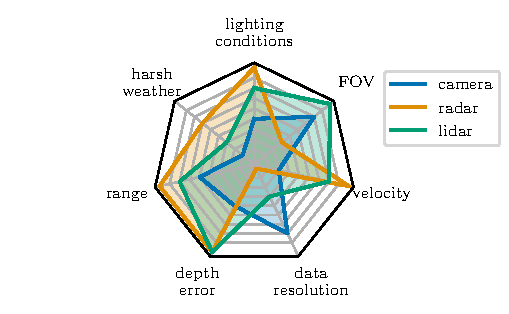
\includegraphics{img/spider_sensorcomp.pdf}
\centering
\caption{Figures MUST be in PDF (everything that can be a vector must be a vector) or PNG format to prevent issues with the arXiv upload.}
\label{fig:compare_sensors}
\end{figure}

% \section{Evaluation}
\label{sec:evaluation}


% \section{Conclusion}
\label{sec:conclusion}

Discussion and Outlook
% \section{Acknowledgment}
\label{sec:acknowledgment}

This work results partly from the KIGLIS project supported by the German Federal Ministry of Education and Research (BMBF), grant number 16KIS1231.

% -------------------------- REFERENCES -------------------------------

{\small
\bibliographystyle{IEEEtran}
\bibliography{literature/AllSourcesMHO.bib}
}

\end{document}
